\documentclass[14pt]{extreport}
\usepackage{cmap}
\usepackage[utf8]{inputenc}
\usepackage[english,ukrainian]{babel}
\usepackage{graphicx}
\usepackage{geometry}
\usepackage{listings}
\usepackage{amsmath}
\usepackage{float}
\geometry{
	a4paper,
	left=20mm,
	right=20mm,
	top=20mm,
	bottom=20mm
}
\lstset{
	language=bash,
	tabsize=4,
	breaklines,
	keepspaces,
	showstringspaces=false,
}
\graphicspath{ {./pictures} }
\setlength{\parindent}{4em}

\newcommand\subject{Кросплатформне програмування}
\newcommand\lecturer{доцент кафедри ПЗ\\Дяконюк Л.М.}
\newcommand\teacher{ст. викл. кафедри ПЗ\\Шкраб Р.Р.}
\newcommand\mygroup{ПЗ-32}
\newcommand\lab{6}
\newcommand\theme{Робота з Stream API}
\newcommand\purpose{Навчитися працювати з Stream API}

\begin{document}
\begin{normalsize}
	\begin{titlepage}
		\thispagestyle{empty}
		\begin{center}
			\textbf{МІНІСТЕРСТВО ОСВІТИ І НАУКИ УКРАЇНИ\\
				НАЦІОНАЛЬНИЙ УНІВЕРСИТЕТ "ЛЬВІВСЬКА ПОЛІТЕХНІКА"}
		\end{center}
		\begin{flushright}
			Інститут \textbf{КНІТ}\\
			Кафедра \textbf{ПЗ}
		\end{flushright}
		\vspace{160pt}
		\begin{center}
			\textbf{ЗВІТ}\\
			\vspace{10pt}
			До лабораторної роботи № \lab\\
			\textbf{На тему}: “\textit{\theme}”\\
			\textbf{З дисципліни}: “\subject”
		\end{center}
		\vspace{40pt}
		\begin{flushright}
			
			\textbf{Лектор}:\\
			\lecturer\\
			\vspace{10pt}
			\textbf{Виконав}:\\
			
			студент групи \mygroup\\
			Коваленко Д.М.\\
			\vspace{10pt}
			\textbf{Прийняв}:\\
			
			\teacher\\
			
			\vspace{28pt}
			«\rule{1cm}{0.15mm}» \rule{1.5cm}{0.15mm} 2023 р.\\
			$\sum$ = \rule{1cm}{0.15mm}……………\\
			
		\end{flushright}
		\vspace{\fill}
		\begin{center}
			\textbf{Львів — 2023}
		\end{center}
	\end{titlepage}
		
	\begin{description}
		\item[Тема.] \theme.
		\item[Мета.] \purpose.
	\end{description}
	

	\section*{Лабораторне завдання}
Створити класи для сутностей, описаних в завданні. Наповнити колекції даних
з текстових файлів. Для виконання завдань розробити меню. Для реалізації
використовувати технологію потоків Stream.API. Cеріалізувати колекції.	
	
	Створити класи для бібліотеки. Клас Книга повинен містити інформацію про
	автора, назву та рік видання.
	Клас Абонемент знатиме прізвище, ім’я та по-батькові, а також електронну
	адресу.
	Кожен читач може взяти певну кількість книг, список яких він зберігає.
	Адміністратор фіксує дату, коли читач забирає книгу і дату планового
	повернення, а також дату реального повернення.
	Клас бібліотека містить колекцію всіх книг та колекцію всіх абонементів, а
	також методи, які з цими колекціями можна здійснювати.
	
	Дано текст, який складається з багатьох стрічок. Речення можуть бути в кількох
	стрічках. Вважати, що відсутні перенесення слова.
	\begin{itemize}
\item Відсортувати всі книги за роком видання.
\item Створити список адресів для розсилки повідомлень для читачів, що взяли
більше ніж 2 книги.
\item Перевірити, скільки користувачів взяли книги заданого автора.
\item Знайти найбільшу кількість книг, взятого читачем бібліотеки.
\item Здійснити різну розсилку 2 групам користувачів. У першу групу занести
користувачів, які мають менше 2 книг. Їм повідомити про новинки бібліотеки. У
другу групу занести інших користувачів. Їм повідомити про вчасність повернення
книг.
\item  Створити список боржників на біжучу дату. Для кожного боржника вказати
список книг, які підлягають поверненню, з вказівкою кількості днів порушення
терміну.
	\end{itemize}
	\section*{Хід роботи}

	\textbf{\textit{Main.java}}
	\begin{lstlisting}
import java.io.BufferedReader;
import java.io.FileReader;
import java.io.IOException;
import java.text.ParseException;
import java.text.SimpleDateFormat;
import java.util.*;
import java.util.stream.Collectors;

class Book {
	String author;
	String title;
	int year;
	
	public Book(String author, String title, int year) {
		this.author = author;
		this.title = title;
		this.year = year;
	}
	
	int getYear() {
		return this.year;
	}
	
	@Override
	public String toString() {
		return "Book {" +
			"author='" + author + '\'' +
			", title='" + title + '\'' +
			", year=" + year +
			"}\n";
	}
}

class Subscription {
	String lastName;
	String firstName;
	String email;
	
	public Subscription(String lastName, String firstName, String email) {
		this.lastName = lastName;
		this.firstName = firstName;
		this.email = email;
	}
	
	@Override
	public String toString() {
		return "Subscription{" +
			"lastName='" + lastName + '\'' +
			", firstName='" + firstName + '\'' +
			", email='" + email + '\'' +
			'}';
	}
	// Getters and setters if needed
}

class BorrowedBook {
	String author;
	String title;
	int year;
	Date borrowDate;
	Date plannedReturnDate;
	Date actualReturnDate;
	
	public BorrowedBook(String author, String title, int year, Date borrowDate, Date plannedReturnDate, Date actualReturnDate) {
		this.author = author;
		this.title = title;
		this.year = year;
		this.borrowDate = borrowDate;
		this.plannedReturnDate = plannedReturnDate;
		this.actualReturnDate = actualReturnDate;
	}
	
	@Override
	public String toString() {
		return "BorrowedBook{" +
			"author='" + author + '\'' +
			", title='" + title + '\'' +
			", year=" + year +
			", borrowDate=" + borrowDate +
			", plannedReturnDate=" + plannedReturnDate +
			", actualReturnDate=" + actualReturnDate +
			'}';
	}
	// Getters and setters if needed
}
class Reader {
	Subscription subscription;
	List<BorrowedBook> borrowedBooks;
	Date actualReturnDate;
	Date plannedReturnDate;
	public Reader(Subscription subscription, List<BorrowedBook> borrowedBooks) {
		this.subscription = subscription;
		this.borrowedBooks = borrowedBooks;
	}
	
	@Override
	public String toString() {
		return "Reader{" +
			"subscription=" + subscription +
			", \n\tborrowedBooks=" + borrowedBooks +
			"}\n";
	}
	// Getters and setters if needed
}

class Library {
	List<Book> allBooks;
	List<Reader> allReaders;
	
	public Library(List<Book> allBooks, List<Reader> allReaders) {
		this.allBooks = allBooks;
		this.allReaders = allReaders;
	}
	
	// Task 1: Sort all books by the year of publication
	public List<Book> sortBooksByYear() {
		return allBooks.stream().sorted(Comparator.comparingInt(Book::getYear)).collect(Collectors.toList());
	}
	
	// Task 2: Create a list of addresses for heavy readers
	public List<String> getAddressesForHeavyReaders() {
		return allReaders.stream()
		.filter(reader -> reader.borrowedBooks.size() > 2)
		.map(reader -> reader.subscription.email)
		.collect(Collectors.toList());
	}
	
	// Task 3: Check how many users took books from a specified author
	public long countUsersByAuthor(String author) {
		return allReaders.stream()
		.flatMap(reader -> reader.borrowedBooks.stream())
		.filter(book -> book.author.equals(author))
		.count();
	}
	
	// Task 4: Find the maximum number of books taken by a reader
	public int getMaxBooksTakenByReader() {
		return allReaders.stream()
		.mapToInt(reader -> reader.borrowedBooks.size())
		.max()
		.orElse(0);
	}
	
	// Task 5: Send different messages to two groups of users
	public void sendMessagesToUsers() {
		List<Reader> group1 = allReaders.stream()
		.filter(reader -> reader.borrowedBooks.size() < 2)
		.toList();
		
		List<Reader> group2 = allReaders.stream()
		.filter(reader -> reader.borrowedBooks.size() >= 2)
		.toList();
		
		// Implement sending messages to each group
		System.out.println("Group 1: Notify about new library arrivals");
		group1.forEach(reader -> System.out.println("Message to " + reader.subscription.email + ": New library arrivals"));
		
		System.out.println("\nGroup 2: Remind about timely book returns");
		group2.forEach(reader -> System.out.println("Message to " + reader.subscription.email + ": Return books on time"));
	}
	
	// Task 6: Create a list of debtors and their overdue books
	public Map<Reader, List<BorrowedBook>> getDebtors() {
		Date currentDate = new Date();
		
		return allReaders.stream()
		.filter(reader -> reader.actualReturnDate == null || (reader.actualReturnDate.after(reader.plannedReturnDate) && reader.actualReturnDate.after(currentDate)))
		.collect(Collectors.toMap(
		reader -> reader,
		reader -> reader.borrowedBooks.stream()
		.filter(borrowedBook ->
		borrowedBook.actualReturnDate == null ||
		(borrowedBook.actualReturnDate != null &&
		borrowedBook.plannedReturnDate != null &&
		borrowedBook.actualReturnDate.after(borrowedBook.plannedReturnDate) &&
		borrowedBook.actualReturnDate.after(currentDate)))
		.collect(Collectors.toList())
		));
	}
	
	
	
	// New method to parse borrowed book data
	private BorrowedBook parseBorrowedBook(String[] data) throws ParseException {
		String readerEmail = data[1];
		Reader reader = allReaders.stream()
		.filter(r -> r.subscription.email.equals(readerEmail))
		.findFirst()
		.orElseThrow(() -> new IllegalArgumentException("Reader not found for borrowed book entry."));
		
		String author = data[2];
		String title = data[3];
		int year = Integer.parseInt(data[4]);
		
		SimpleDateFormat sdf = new SimpleDateFormat("yyyy-MM-dd");
		Date borrowDate = sdf.parse(data[5]);
		Date plannedReturnDate = data[6].isEmpty() ? null : sdf.parse(data[6]);
		Date actualReturnDate = data[7].isEmpty() ? null : sdf.parse(data[7]);
		
		return new BorrowedBook(author, title, year, borrowDate, plannedReturnDate, actualReturnDate);
	}
	
	
	// New method to read borrowed book entries from file
	List<BorrowedBook> readBorrowedBooksFromFile(String filePath) {
		List<BorrowedBook> borrowedBooks = new ArrayList<>();
		Reader currentReader = null;
		
		try (BufferedReader br = new BufferedReader(new FileReader(filePath))) {
			String line;
			while ((line = br.readLine()) != null) {
				String[] data = line.split(",");
				if ("Reader".equals(data[0])) {
					if (currentReader != null) {
						allReaders.add(currentReader);
					}
					currentReader = new Reader(new Subscription(data[1], data[2], data[3]), new ArrayList<>());
				} else if ("BorrowedBook".equals(data[0]) && currentReader != null) {
					BorrowedBook borrowedBook = parseBorrowedBook(data);
					currentReader.borrowedBooks.add(borrowedBook);
					borrowedBooks.add(borrowedBook);
				}
				// Add more conditions for other types of data if needed
			}
			// Add the last reader to the list
			if (currentReader != null) {
				allReaders.add(currentReader);
			}
		} catch (IOException | ParseException e) {
			e.printStackTrace();
		}
		
		return borrowedBooks;
	}
}

public class Main {
	public static void main(String[] args) {
		List<Book> allBooks = new ArrayList<>();
		List<Reader> allReaders = new ArrayList<>();
		
		try (BufferedReader br = new BufferedReader(new FileReader("./src/library_data.txt"))) {
			String line;
			while ((line = br.readLine()) != null) {
				String[] data = line.split(",");
				if ("Book".equals(data[0])) {
					allBooks.add(new Book(data[1], data[2], Integer.parseInt(data[3])));
				} else if ("Reader".equals(data[0])) {
					allReaders.add(new Reader(new Subscription(data[1], data[2], data[3]), new ArrayList<>()));
				}
				// Add more conditions for other types of data if needed
			}
		} catch (IOException e) {
			e.printStackTrace();
		}
		
		Library library = new Library(allBooks, allReaders);
		
		library.readBorrowedBooksFromFile("./src/library_data.txt");
		
		Scanner scanner = new Scanner(System.in);
		
		while (true) {
			System.out.println("\nSelect a task to perform:");
			System.out.println("1. Sort all books by the year of publication");
			System.out.println("2. Create a list of addresses for heavy readers");
			System.out.println("3. Check how many users took books from a specified author");
			System.out.println("4. Find the maximum number of books taken by a reader");
			System.out.println("5. Send messages to users");
			System.out.println("6. List of debtors and overdue books");
			System.out.println("0. Exit");
			
			int choice = scanner.nextInt();
			scanner.nextLine(); // Consume newline character
			
			switch (choice) {
				case 1:
				System.out.println("Task 1: Sorted books by year: \n" + library.sortBooksByYear());
				break;
				case 2:
				System.out.println("Task 2: Addresses for heavy readers: " + library.getAddressesForHeavyReaders());
				break;
				case 3:
				System.out.print("Enter author name: ");
				String authorName = scanner.nextLine();
				System.out.println("Task 3: Users who took books from " + authorName + ": " + library.countUsersByAuthor(authorName));
				break;
				case 4:
				System.out.println("Task 4: Maximum number of books taken by a reader: " + library.getMaxBooksTakenByReader());
				break;
				case 5:
				System.out.println("Task 5: Sending messages to users: \n");
				library.sendMessagesToUsers();
				break;
				case 6:
				System.out.println("Task 6: List of debtors and overdue books: \n" + library.getDebtors());
				break;
				case 0:
				System.out.println("Exiting the program.");
				System.exit(0);
				default:
				System.out.println("Invalid choice. Please enter a valid option.");
			}
		}
	}
}

	\end{lstlisting}	
	
	\begin{figure}[H]
		\centering
		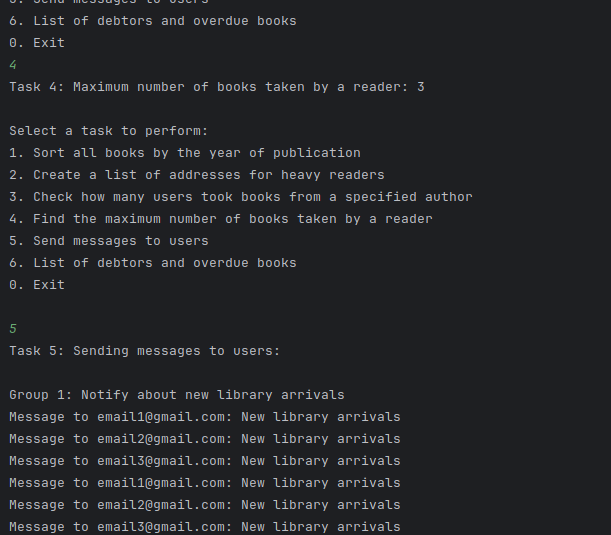
\includegraphics[scale=0.55]{1}
		\caption{Робота програми}
	\end{figure}

	\section*{Висновок}
	Під час виконання лабораторної роботи я працював з Stream API. Навчився працювати з Stream API.
	 
\end{normalsize}
\end{document}
